\Chapter{Kínai karakterek felismerése}

{\large \textbf{Az alapvonások}}

Az írásjegyek felépítésének következő lényeges szabálya az írásjegy vonásainak sorrendje. Az írásjegyek – bármilyen bonyolult legyen is némelyik – tulajdonképpen néhány igen egyszerű vonalból épülnek fel. Ezek az írásjegyek alapelemei, vagy alap-ecsetvonásai. A jobb oldali képen az alapvonások néhány főbb típusa látható. Természetesen az alapvonásoknak több változata is lehetséges (méret, vastagság, irány) attól függően, hogy az írásjegy melyik részén helyezkedik el.

\begin{center}
	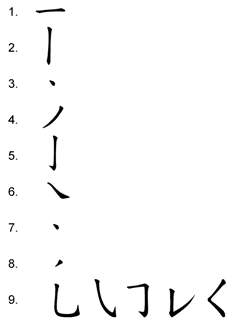
\includegraphics[width=0.4\linewidth]{images/chinese_strokes.png}
\end{center}



Minden egyes vonásnak megvan a felépítési szabálya: az ecsetvonásoknak meghatározott sorrendben kell követniük egymást, mégpedig általános elvként az írásjegyek határait alkotó virtuális négyszög bal felső sarkából lefelé és jobbra haladva. Az írásjegy gerincét, fő szerkezeti elemét adó nagyobb vonást, ha az egész írásjegyet átjárja, legutoljára húzzák.

\newpage
{\large \textbf{A vonássorrend szabályai: }}
\begin{enumerate}
	\item A vízszintes vonások megelőzik a függőleges vonásokat.
	\item A balra lejtő vonások megelőzik a jobbra lejtő vonásokat. 
	\item Az írásjegyek írását felülről kell kezdeni. 
	\item Az írásjegyet balról jobbra haladva építik fel. 
	\item A felülről keretezett írásjegyeknél előbb a keretet kell meghúzni. 
	\item Az alulról keretezett írásjegyeknél a keretet legvégül kell meghúzni. 
	\item A teljes keretet mindig legvégül kell bezárni.
\end{enumerate}

Egy szimmetrikus felépítésű írásjegynél előbb a középső részt kell kialakítani, s csak azután az oldalakat.

\begin{center}
	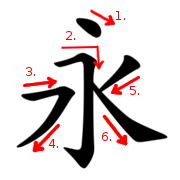
\includegraphics[scale=1.0]{images/vonasrend_ordered.png}
\end{center}

A kínai írásjegyek különböző számú alapvonásokból épülhetnek fel. Ezek közül a legegyszerűbb a csupán egyetlen vízszintes vonalból álló „egy” jelentésű \begin{CJK*}{UTF8}{gbsn}
一
\end{CJK*} ji írásjegy. A kínai írásrendszer más, egy vonásból álló írásjegyet nem tartalmaz. Aránylag ritkák a két vonásból álló írásjegyek is, például: \begin{CJK*}{UTF8}{gbsn}
二
\end{CJK*} er„kettő”,
\begin{CJK*}{UTF8}{gbsn}
十
\end{CJK*} si „tíz”,
\begin{CJK*}{UTF8}{gbsn}
人
\end{CJK*} zsen „ember” stb. A hagyományos írásjegyek zöme 15–30 vonásból épül fel (átlagosan 9 vonásból). Esetenként azonban ennél jóval több vonásból álló írásjegyek is előfordulhatnak, melyek tulajdonképpen már több önálló írásjegy összevonásának is tekinthetők. Ritkák ugyan, de léteznek 50 vagy akár 80 vonásból álló írásjegyek is.\\

{\Large OCR megvalósítások}

A következőkben bemutatok néhány olyan alkalmazást, amelyek az optikai karakterfelismerés egyes részeit hivatottak megvalósítani. Ezek között szerepelnek olyanok, amelyek meglehetősen szűk témakörrel, például számjegyek felismerésével foglalkoznak, de lesznek olyanok is, amelyek meglehetősen komoly eredményeket képesek felmutatni a kézírásos karakterek felismerése terén. Minden esetben részletesen kitérek arra, hogy az alkalmazás készítése során milyen megfontolások vezettek az adott neurális hálózat felépítésének megválasztásához, bemutatom az egyes területeken megjelenő és kezelendő problémákat, illetve összehasonlításokkal és adatokkal támasztom alá az egyes rendszerek hatékonyságát és alkalmazhatóságát a kijelölt problémára. 

Számjegyek felismerése zajos képeken 

A zajos számjegyek és karakterek a rendszámtáblák felismerésénél általános jelenségnek számítanak, mivel itt a kamera felvétele általában mozgó járműről készül, és a zajt tovább növelheti a piszok, a nedves, esetleg esős időjárás, éjszakai sötétség, a tükröződés stb. Jelen esetben tekintsünk el a különböző felvételi körülmények által okozott természetes hibáktól és vizsgáljuk meg, milyen eredménnyel ismerünk fel mesterségesen eltorzított képeken számjegyeket. A beolvasott képeket a következő módszerekkel tesszük zajosabbá: 

\begin{itemize}
\item Gauss zajok alkalmazásával. 
\item Képfeldolgozási eszközök használatával (elmosás). 
\item Véletlenszerűen részletek kitörlésével. 
\end{itemize}

Mivel a program hatékonyságát nagymértékben befolyásolja a neurális hálózat felépítése, gondosan meg kell terveznünk, hogy milyen hálózatot alkalmazunk az egyes problémák megoldásához. Jelen esetben az átlagos négyzetes hiba (MSE) segítségével értékeljük a hálózat hatékonyságát és több hálózat teljesítményét összevetve választjuk ki, hogy milyen felépítést használunk a jelenlegi problémánkhoz. 

Első lépésben ki kell választanunk a rejtett és a kimeneti réteg neuronjai által alkalmazott aktivációs függvényt. Jelen esetben a rejtett rétegbeli neuronoknál tangens szigmoid, a kimeneti réteg neuronjainál pedig logaritmus szigmoid függvényt alkalmazunk. 

Természetesen lehetőségünk lenne akár minden rejtett rétegbeli neuronnál, illetve minden kimeneti neuronnál ugyanazt vagy akár mindegyiknél különböző aktivációs függvényt használni, de jelen esetben, a négyzetes hiba mértékét figyelembe véve ez a két függvény megfelelőnek látszik arra, hogy a segítségével a neurális hálózatunk nagy hatékonysággal ismerje fel az egyes számjegyeket. 

A következő táblázatból látszik, hogy nem lehet egyértelműen megmondani, hogy az egyes neuronszámok mellett milyen hibaértékek várhatók. A táblázatból az is kitűnik, hogy 9 rejtett neuronnal a négyzetes hibát látványosan kisebbre lehetett visszaszorítani. 

\begin{center}
\begin{tabular}{ |c|c|c| } 
 \hline
 Rejtett neuronok száma  & MSE  \\ 
 \hline\hline
 1 & 0,1424 \\
 \hline
 2 & 0,0485 \\
 \hline
 3 & 0,0508 \\
 \hline
 4 & 0,0745 \\
 \hline 
 5 & 0,0809 \\
 \hline
 6 & 0,0933 \\
 \hline
 7 & 0,1183 \\
 \hline 
 8 & 0,0386 \\
 \hline
 9 & $1,9509*10^{-12}$ \\
 \hline
 10 & 0,0039 \\
 \hline
 11 & 0,1691 \\
 \hline
 12 & 0,0025 \\
 \hline
 13 & 0,0014 \\
 \hline
 14 & 0,0014 \\
 \hline
\end{tabular}
\end{center} 

A neurális hálózat ideális felépítésének meghatározása után a következő lépés a tanulóhalmaz összeállítása. A számjegyek felismerésére készített hálózatot a következő tanulópéldákkal tanítjuk be: 

\begin{itemize}
\item Normál számok 
\item Háromszor és tizenkétszer elmosott számok 
\item Öt és harminc közötti intenzitású Gauss zajjal módosított számok
\item Kézzel írt karakterek felismerése
\end{itemize}

Az előbbi példából látszik, hogy a számjegyek felismerése egyszerű folyamat. A kézírásos karakterek felismerése jóval nehezebb, hiszen gyakorlatilag nem támaszkodhatunk arra, hogy egy adott karakterkészletből kell kiválasztanunk a megfelelő betűt. A kézírások változatosságából adódóan nagyon körültekintően kell megválasztanunk, hogy milyen módszert, illetve milyen felépítésű neurális hálózatot használunk, hiszen nem csak a felismerés hatékonyságát, hanem a rendszer betanítási és futási idejét is figyelembe kell vennünk. 

Ebben a részben egy olyan neurális háló alkalmazással ismerkedünk meg, amely már kézzel írt karaktereket kap bemenetként és ezek felismerésére tesz kísérletet. 

A kézzel írt karakterek felismerésének első lépéseként a felismerni kívánt karaktereket szeparálni kell a képen található többi információtól, illetve a szavakat, szókapcsolatokat karakterekre kell bontani. A kép ilyen formájú feldolgozása után az egyes karaktereket tartalmazó képeket digitalizálni kell. A digitalizálás folyamán a képekből egy bináris mátrix készül. Minden fekete pixelnek egyest, minden fehérnek nullát feleltetünk meg. 

A következő ábrán látható, hogy milyen lépések folyamán jutunk el a kézzel írt A betűtől addig a bitmátrixig (I), amelyet a neurális hálózat már értelmes bemenetként képes kezelni. A digitalizálás folyamán minden karaktert ugyanakkora méretűvé alakítunk, így a hálózat minden esetben egy előre meghatározott méretű bitmátrixszal dolgozik majd. 